\section{Client}\label{sec:client}

The client application is substantially a collection of menus and forms. Each
menus creates a list of entries and when the user selects an entry the
corresponding handler (a method) is called. Forms validate every input that the
user inserts.

The crafting of the requests to submit to the server is made by the
\code{Protocol} class. Beside that, the client only implements presentation
logic.

A guide to use the client can be found in \chref{ch:manual}.

\figref{fig:client} shows the class diagram for the Client. Only the main
classes are shown.

\begin{figure}[htb]
	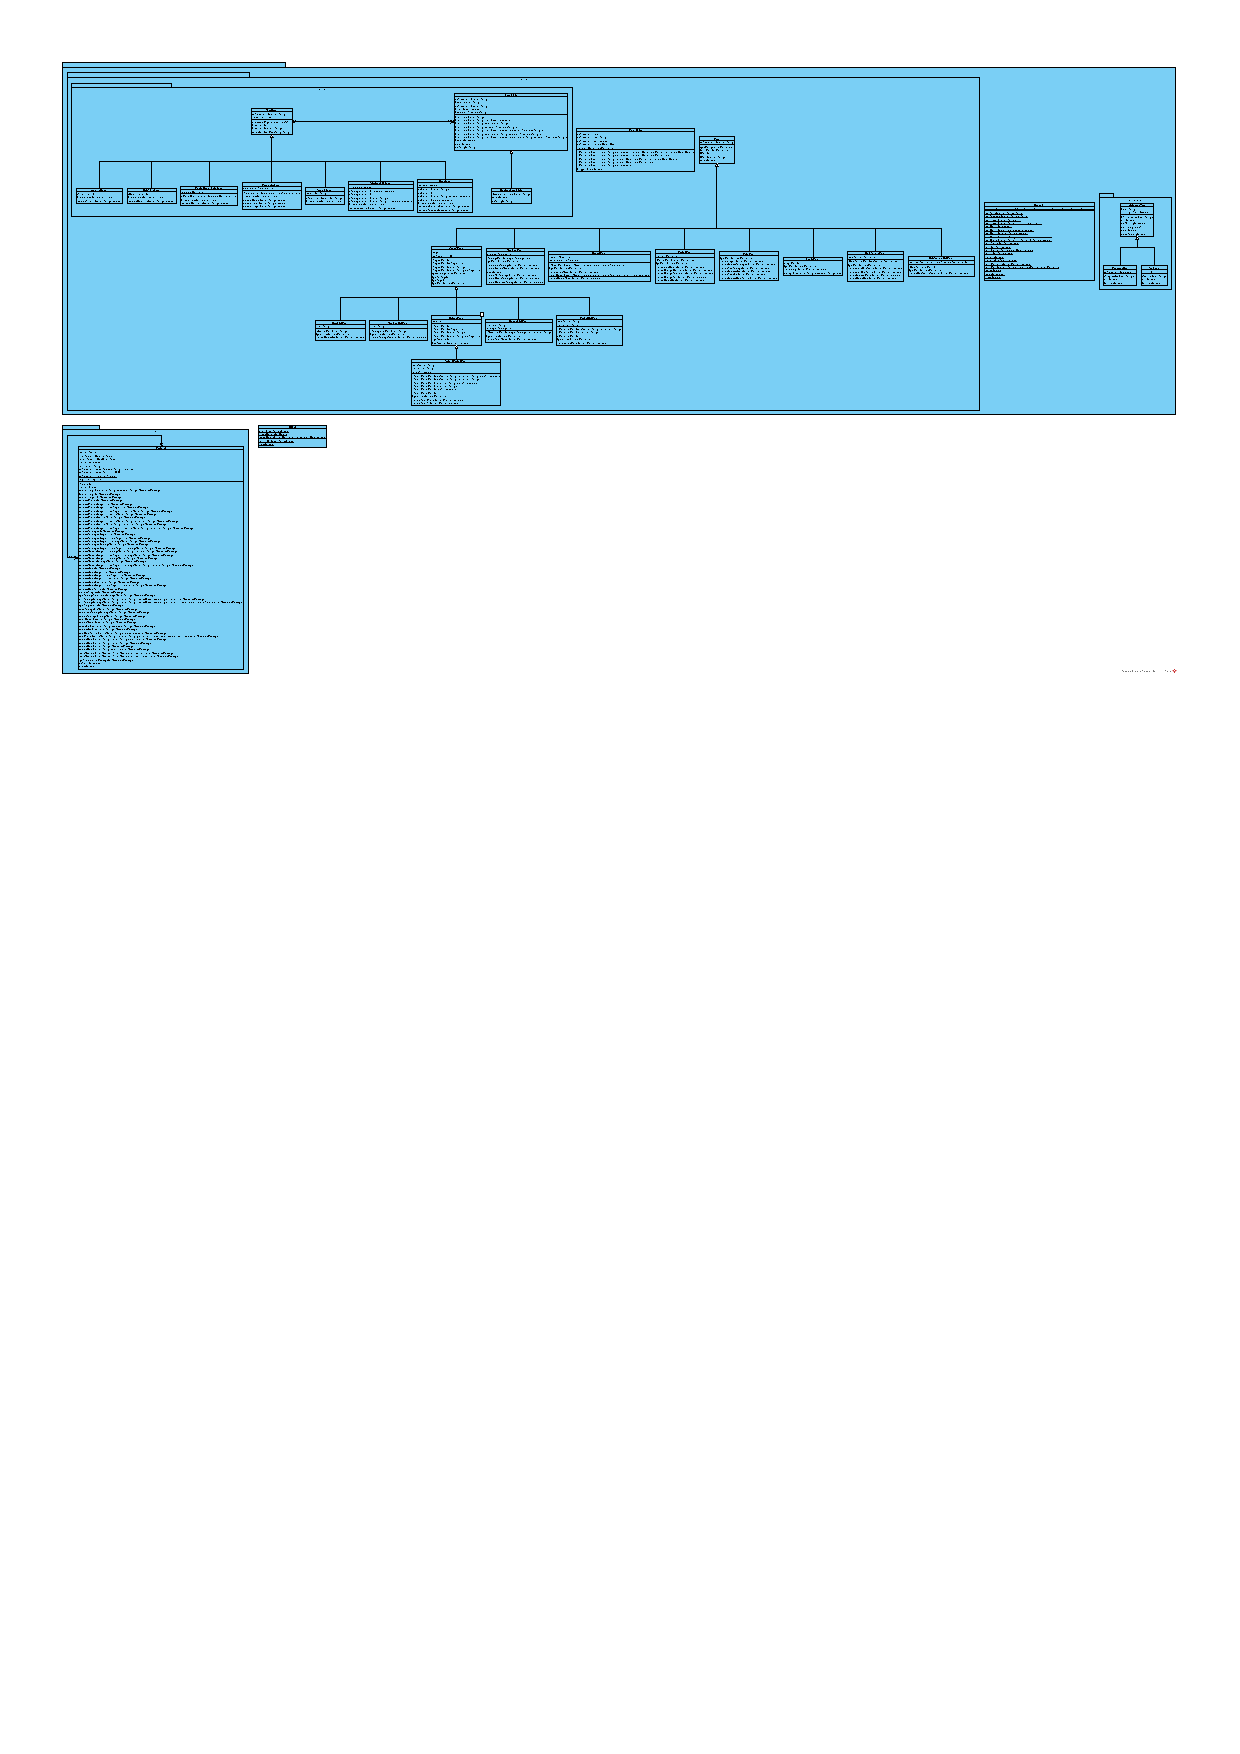
\includegraphics[width=\textwidth]{module-client}
	\caption{Client class diagram.}\label{fig:client}
\end{figure}
